\subsection{A brief history of Roman numeral analysis}
\label{sec:a_brief_history_of_roman_numeral_analysis}

\guide{What do we call Roman numeral analysis?}
Roman numeral analysis is a common methodology in contemporary music theory textbooks dealing with tonal music.
The name derives from the use of Roman numerals to denote scale degrees, which, in turn, indicate diatonic chords in a certain key context.

\guide{Why is Roman numeral analysis important compared to, say, chord labels?}
Roman numeral labels provide more information than chord labels.
Generally, a chord label indicates the root of a chord and its quality.
A Roman numeral label provides this as well, but also information about keys, inversions, and spellings.
For example, Roman numerals are always relative to a key, so the key must be indicated at all times to disambiguate the meaning of the Roman numeral.
This is a helpful property for passages of music that feature quick modulations or changes of key.
In the modern syntax, it is also customary to indicate \emph{applied chords} or \emph{secondary dominants}.
Once the concept of \emph{tonicization} emerged, in the twentieth century, this quickly became an important idea of tonal music, particularly relevant to analyze the chromatic music of the nineteenth century.
Roman numerals facilitate the indication of modulations as well as tonicizations.
With these, a musical analysis of a particular person can be more informative, for example, indicating how the analyst envisions the key context at a particular moment of the piece.
Roman numerals indicate inversions for triads and seventh chords.
Presumably, the Arabic numeral notations employed to denote inversions in Roman numerals evolved from figured bass.
However, there is generally a small vocabulary of numerical annotations appended to a Roman numeral, which indicate the inversion of the chord.
There are other subtle but important differences that come with Roman numeral analysis compared to chord labels.
Think of a diminished seventh chord, say, F$\sharp$ diminished seventh.
The most usual context of that chord is to anticipate a resolution to a G minor triad.
However, if the chord is in first inversion, then it is enharmonically equivalent to an A diminished seventh chord.
It is tempting to write the chord as A diminished, rather than F$\sharp$ with A in the bass, however, these chords have two very different meanings contextually.
This is evident in the presence of pitch spelling.
The G$\flat$--G$\natural$ results in a strange voice leading, whereas the F$\sharp$--G is a customary leading-tone to tonic minor second.
These subtle interactions of spelling are generally honored by the Roman numeral analysis notation.
There are multiple examples that come to mind, such as Neapolitans, Augmented Sixth Chords, and \emph{Cadential six-four} chords, where the syntax of Roman numerals is helpful to provide a more thorough description of the annotated chord.
These differences might seem negligible to some, but I would like to make a few arguments: (1) in tonal music theory textbooks, it is more common to see Roman numeral analysis notation than chord labels, which might suggest that the more granular notation is preferred (2) in machine learning contexts, as is the case for this dissertation, more information in the annotations can be really helpful, without this additional information, we could not attempt to learn a key-estimation model simultaneously using the same annotated data, (3) the syntax of Roman numeral analysis is highly compressed, it is generally not more time-consuming to write Roman numerals than it is to write chord labels, the time-consuming aspect of Roman numerals is the train of thought required to commit to a particular interpretation of the analysis (i.e., key context, chord, inversion, function of the chord), and that is precisely the thorough thought pattern that we want to capture in the data.


\guide{How did Roman numeral analysis emerge?}
It is problematic to pinpoint a time and place where this notational system appeared.
It seems more accurate to say that this notation did not ``appear'' but evolved, slowly, from the sporadic use of Roman numerals indicating scale degrees, to the complex syntax of applied chords and chord inversions used today.

In this section, I summarize a brief timeline of this evolution process.
For describing the important developments that lead to our modern Roman numeral analysis notation, I rely on existing literature.
For example, the chapters on tonality of the Cambridge History of Western Music Theory~\parencite{christensen_tonality_2002, christensen_rameau_2002, christensen_nineteenth-century_2002, christensen_heinrich_2002}.
The historical events discussed by previous scholars are complemented with a timeline of Roman numeral analysis syntax that I collected from different textbooks of the nineteenth century.

\guide{Important developments that lead to the modern Roman numeral analysis syntax.}
There are a few historical figures who influenced the notation that we know today.
Rameau's fundamental bass, Vogler's first use of Roman numerals, Weber's notation for Roman numerals with chord qualities (big case for major triads, small case for minor triads, circle postfix to denote diminished triads), Riemann's concept of function and applied chords, Schoenberg's take on function, Schenker's tonicization.

\guide{Rameau's fundamental bass.}
When I was introduced to tonal harmony in school, Rameau was introduced as the \emph{father of Harmony}.
When I took this course, I was well aware of Rameau's music as well as Bach's.
I used to listen to the Harpsichord pieces of both composers, as the harpsichord was my favorite instrument.
Something that was very confusing for me was how the music by previous composers seemed to have ``chords''.
How is it that Rameau is the ``father of harmony''? I am pretty sure I have heard chords in earlier composers.
There seemed to be a lot of misinformation and ``myths'' in music theory.
Over the years, I managed to confirm this over and over.
The \emph{meaning} of a certain key, the nonexistence of ``parallel fifths'' in music from the ``great masters'', and on and on.
Nowadays, I have reconciled my thoughts on this particular topic, Rameau as the ``father of Harmony''.
The concept of ``chord root'' is taken for granted nowadays, as a universal phenomenon of Western tonal music.
Even when approaching Fuxian counterpoint theory, music teachers have for many years relied on the concept of ``the root'' to analyze triads and seventh chords formed from contrapuntal motion.
This concept, the chord root, is highly correlated with the idea of the ``fundamental bass'', introduced by Rameau.
A good explanation is found in~\textcite{christensen_rameau_2002}.
In the times of figured bass, a bass with an annotation of ``6'' indicated a harmony that was more closely linked to ``5'' than it was to its own ``chord root''.
How we would think of it today.
For example, a C major triad is not as related to an A minor triad in first inversion as it is to a C major triad in first inversion or second inversion, even though the bass of ``C:I'' and ``a:i6'' is potentially the same.
The root is important, more than the bass.
This is what the ``fundamental bass'' revolution brought to music theory and, according to other scholars, it changed everything.
I agree, and I accept Rameau as an essential figure in this process now.


It has been customary to divide the different tonal theories of harmony of the eighteenth and nineteenth centuries into two branches: \emph{scale-degree} theories and \emph{functional} theories.

The difference between these groups is that the functional theories tend to attempt explanations for the ``role'' or ``function'' that a chord has in a specific context, whereas the scale-degree theories tend to focus on the more objective chord ``root'', without too much explanation of the context or the role of this scale degree.

The modern Roman numeral analysis syntax tends to borrow ideas from these two branches of theories, as it sometimes indicates functional aspects.
For example, the label `V/V`, which is common in Roman numeral analysis could also be indicated as `II'.
Assuming that the notation is case-sensitive, the upper case `II' indicates a major triad on the second degree, which is the correct root and chord quality of the chord indicated by `V/V'.
By indicating the chord as `V/V', implicitly, there is some contextual information being introduced into the label.
Namely, the notation indicates that this chord has possibly some relationship to a chord that will happen in the future (a dominant), and it is acting as a dominant chord for it (thus, ``dominant of the dominant'').

Although this hybrid nature of modern Roman numerals is not often discussed, it seems customary nowadays in textbooks, explanations, and general understanding of tonal music theories of the past.


\guide{Vogler's first use of Roman numerals.}
Except for the nonexistence of zero, there is nothing special about Roman numerals, per se.
They are symbols that can be used to count natural numbers.
Vogler used them for this purpose in 177X.
More precisely, to refer to the seventh degree of a major diatonic scale (i.e., the leading tone).
In a subsequent work in 1802, Vogler used Roman numerals to denote each scale degree similarly.
This was the first use of Roman numerals for this purpose.
An interesting side effect of using the Roman numeral symbols for these annotations, is that Vogler and other authors could also use Arabic numerals to annotate figured bass annotations.
The evidence I have found in textbooks of the nineteenth century suggests that it was common for authors to write figured bass and Roman numerals for the same music excerpt.
Sometimes, these annotations would overlap (e.g., annotating certain chords, such as, augmented sixth chords, using Arabic numerals (figured bass) rather than Roman numerals).
This was a very common practice I observed.
Arguably, this was the reason why the notation evolved to denote chord inversions using Arabic numerals nowadays.

\guide{Weber's notation for Roman numerals.}
Weber is credited with at least two important contributions to music theory: (1) the \emph{tonal chart} table, which was later revisited by Schoenberg and others to measure key relationships, (2) the use of an early Roman numeral notation, which can be considered an early version of the notation used today.
The syntax of Weber is more sophisticated than the one used by Vogler in several aspects.
First, Weber was unequivocally using Roman numerals to denote \emph{chords}, not just scale degrees.
The intention is clear because Weber used bigger (nowadays, upper case) Roman numerals to denote major triads, smaller (nowadays, lower case) Roman numerals to denote minor triads, and a special symbol (``$^{\text{o}}$'') to denote diminished triads, which is still in use today.
That is, the compact notation is now capable of encoding basic chord qualities.
The scale degrees can now be thought as the roots of a chord, where the size (nowadays, case) of the Roman numeral indicates the quality of the triad.

\guide{Riemann.}
Although Rameau first introduced the concepts of Dominant and SubDominant, Riemann introduced them in the context of ``functions''.
In Riemann's theory, three chords (tonic, subdominant, and dominant) were transformed into other chords by applying certain operations.
Although most of Riemann's theory has been left out of modern Roman numeral syntax, his ideas of function and, particularly, concepts of \emph{applied chords} have arguably inspired some aspects of the modern notation.
For example, the use of annotations such as `V/V' have a functional touch to them.
While in scale-degree theories it is customary to describe chords based on the chord root that generates them, the notation of \emph{applied chords} includes more information about neighboring harmonies.
I consider this a functional trait of the notation, because it indicates not only the root and quality of a given chord, but what is its role in the harmonic context.

\guide{Schoenberg.}
Schoenberg revisited the concept of function.
Schoenberg never used the ``V/V'' notation.

\guide{Schenker.}
Schenker is a complicated character, not only in the way he approached music theory but as well on his political views.
Nevertheless, his contributions to music theory are undeniable, and best described by other scholars, such as \textcite{christensen_heinrich_2002}.
The aspects of Schenker that are most relevant for this chapter are his coining of the term ``tonicization'', which is an important trait of modern Roman numeral analysis syntax.

\guide{How does the evolution of Roman numerals look like?}

\begin{itemize}
    \item According to Hyer, there are two branches of tonal music theory around the early nineteenth century: scale-degree theories and functional theories
    \item Scale-degree theories are best characterized by the work of Weber and Schenker
    \item Functional theories include those of Rameau and Riemann
    \item Roman numerals, nowadays unify concepts from these two theories, acting as a metalanguage
    \item Combination of theories is common, for example, Fuxian theory taught by first analyzing the harmonic context of the C.F., and other examples
    \item Arguable, Rameau's work influenced every other subsequent harmonic theory
    \item Rameau introduced the concepts of tonic, dominant, and subdominant chords
    \item However, he never used the term ``function'', which was established by Riemann
    \item Vogler introduced Roman numerals for the first time
    \item First, in 17XX, where he used them to denote the ``VII'' degree
    \item Then, 1802, he used them for every scale degree
    \item Weber firmly established Roman numerals
    \item Nowadays, Roman numerals have borrowed ideas from both branches of music theories
\end{itemize}

\guide{About the timeline.}
In this section, I present a summary of Roman numeral analysis notation across one hundred thirty-three primary sources between the late eighteenth century and early twentieth century.

The primary sources were collected from three keyword searches in the \emph{worldcat} library catalog.
The three keywords are: \emph{harmony}, \emph{harmonie}, and \emph{harmonielehre}.
These keywords were used to search for books in English, French, and German, respectively.
For books with multiple editions, the earliest available\footnote{Physically available at the McGill Marvin Duchow Library, or digitally available in e-book form.} edition was preferred.

The objective of reviewing the resulting primary sources was to observe the evolution of the Roman numeral analysis syntax across harmony textbooks.
Only the musical examples (e.g., an annotated musical staff) were taken into account.
The review was centered around Roman numeral annotations and figured bass.

\textcite{kirnberger1774kunst} introduced the first Roman numeral annotations that indicated scale-degree relationships.
These appeared in two tables of \emph{Die Kunst der reinen Satzes in der Musik}, shown in Figure~\ref{fig:kirnberger1774kunst015}

\begin{figure}[h!]
    \centering
    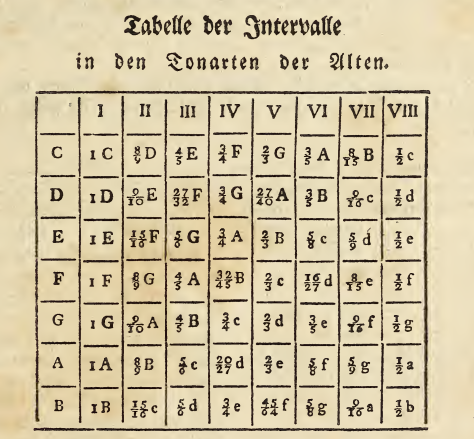
\includegraphics[width=0.6\textwidth]{figures/chapter/2/primary_sources/kirnberger1774kunst015.png}
    \caption{Roman numerals in \textcite{kirnberger1774kunst}.}
    \label{fig:kirnberger1774kunst015}
\end{figure}

Later, \textcite{vogler1778grunde, vogler1802handbuch} introduced the first Roman numeral symbols underneath a staff to indicate scale degrees.
These are used a few times on both works.
Figure~\ref{fig:vogler1778grunde021} shows an example in \textcite{vogler1778grunde}

\begin{figure}[h!]
    \centering
    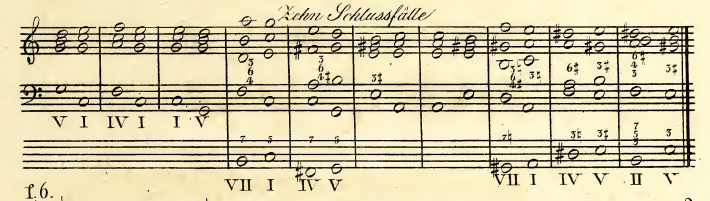
\includegraphics[width=0.6\textwidth]{figures/chapter/2/primary_sources/vogler1778grunde021.png}
    \caption{Roman numerals in \textcite{vogler1778grunde}.}
    \label{fig:vogler1778grunde021}
\end{figure}

While it is difficult to credit someone with ``inventing'' Roman numeral analysis, the modern notation would probably not exist without the precedent of \textcite{weber1817versuch}.
Weber extended the notation to indicate not only scale degrees but their chord quality.
A special notation separates diminished triads (i.e., the seventh degree) from major and minor chords; whereas major and minor are distinguished by the size of the Roman numeral.
Weber introduced several other traits of modern Roman numeral analysis.
Changes of key are indicated using a colon (``:''), multi-layered analyses with several rows of keys and Roman numeral indications.
Finally, whereas previous theorists used the Roman numeral notations sporadically, Weber embraced this notation thoroughly throughout the \emph{Versuch einer geordneten Theorie der Tonsetzkunst} \parencite{weber1817versuch}.
In this book, Weber also indicated dominant seventh chords as $\rn{V}\rnseven$, a notation that is still in use today.
Whereas others relied on figured bass to explain their examples, Weber relied mostly on Roman numerals.

\begin{figure}[h!]
    \centering
    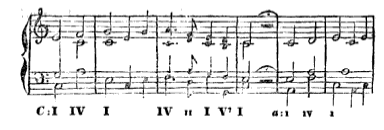
\includegraphics[width=0.6\textwidth]{figures/chapter/2/primary_sources/weber1817versuch205.png}
    \caption{Roman numerals in \textcite{weber1817versuch}. Keys are indicated with colons (e.g., mm. 1 and mm.5). Dominant seventh chords indicated as $\rn{V}\rnseven$. Smaller Roman numerals indicate minor triads.}
    \label{fig:weber1817versuch205}
\end{figure}

After Weber, the first adopter of Roman numerals I could find among my primary sources is \textcite{hamilton1840catechism}.
Hamilton, and several others in the future, did not adopt the case-sensitive notation for chord qualities.
All scale degrees are indicated with a single Roman numeral style, regardless of their chord qualities.
In Hamilton's annotations, Roman numerals indicate melodic scale degrees, instead of chord roots, as shown in Figure~\ref{fig:hamilton1840cathecism044}.

\begin{figure}[h!]
    \centering
    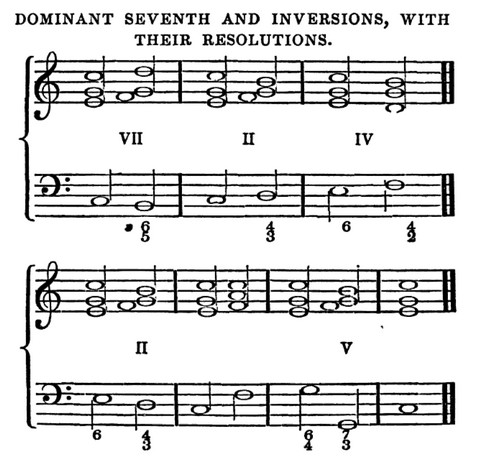
\includegraphics[width=0.6\textwidth]{figures/chapter/2/primary_sources/hamilton1840cathecism044.png}
    \caption{Use of Roman numerals in \textcite{hamilton1840catechism}, indicating the scale degree of the bass, regardless of the chord root. In modern Roman numeral notation, these annotations would be written as $\rn{V}\rnsixfive$, $\rn{V}\rnfourthree$, $\rn{V}\rntwo$, $\rn{V}\rnfourthree$, and $\rn{V}\rnseven$, respectively.}
    \label{fig:hamilton1840cathecism044}
\end{figure}

The next adopter of the Roman numeral notation among German theorists appears to be \textcite{meister1852vollstandige}.
Meister often accompanies the Roman numeral notation with chord labels and figured bass indications, as in Figure~\ref{fig:meister1852vollstandige32}.

\begin{figure}[h!]
    \centering
    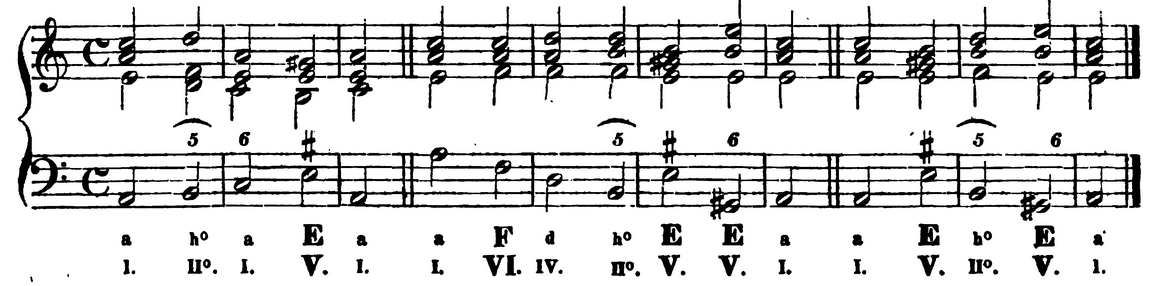
\includegraphics[width=0.6\textwidth]{figures/chapter/2/primary_sources/meister1852vollstandige32.png}
    \caption{Use of Roman numerals in \textcite{meister1852vollstandige}, accompanied by chord label and figured bass indications.}
    \label{fig:meister1852vollstandige32}
\end{figure}

Other authors adopted Roman numerals in the nineteenth century \parencite{sechter1853grundsatze, richter1860lehrbuch, tiersch1874elementarbuch, tracy1878theory}.

An interesting example by \textcite{bussler1878praktische} is shown in Figure~\ref{fig:bussler1878praktische063}, who presents Roman numerals and figured bass annotations in the same analytical layer.
One could claim that this syntax is an early version of the modern chord inversion syntax, where inversions are denoted by stacks of Arabic numerals next to the Roman numeral.

\begin{figure}[h!]
    \centering
    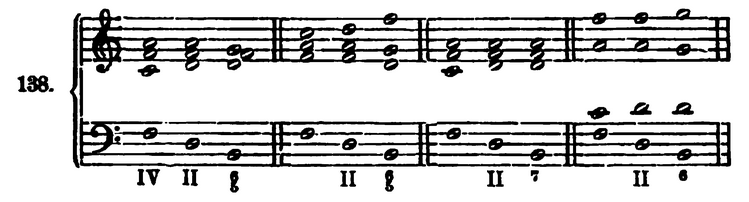
\includegraphics[width=0.6\textwidth]{figures/chapter/2/primary_sources/bussler1878praktische063.png}
    \caption{Use of Roman numerals in \textcite{bussler1878praktische}, accompanied by figured bass indications.}
    \label{fig:bussler1878praktische063}
\end{figure}

This practice is further developed by \textcite{emery1879elements}.
Emery also introduced a special symbol to denote Neapolitan chords, $\rn{N.6}$.
For the augmented sixth chords (i.e., Italian, French, and German), Emery uses a stack of Arabic numerals.
The example shown in Figure~\ref{fig:emery1879elements051} shows this notation. 
Notice that additionally to the stack of Arabic numerals in the layer of Roman numeral analysis, Emery also presents a figured bass layer above the staff.
Lastly, Emery's notation for the augmented sixth quality is the $\rn{+}$ symbol.
Nowadays, this symbol is commonly used to denote augmented triads as well (e.g., $\rn{c:III+}$ in the C harmonic minor scale).
This practice was not conventional around this time.
Up to this point, the notation for modulations is to indicate the changes of key at the level of the Roman numeral annotations. 
A full example of the notation can be seen in another excerpt by Emery, shown in Figure~\ref{fig:emery1879elements102}.

\begin{figure}[h!]
    \centering
    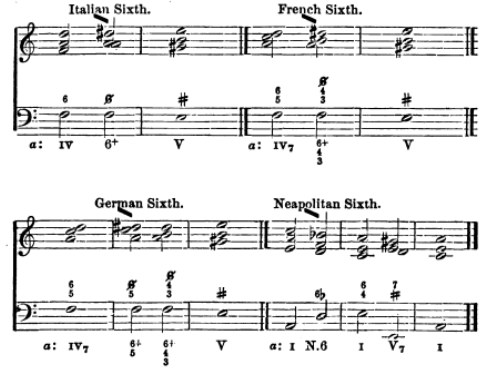
\includegraphics[width=0.6\textwidth]{figures/chapter/2/primary_sources/emery1879elements051.png}
    \caption{Use of Roman numerals in \textcite{emery1879elements}, with notations for Neapolitan chords and augmented sixth chords.}
    \label{fig:emery1879elements051}
\end{figure}

\begin{figure}[h!]
    \centering
    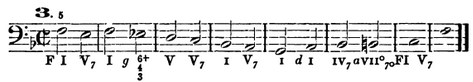
\includegraphics[width=0.6\textwidth]{figures/chapter/2/primary_sources/emery1879elements102.png}
    \caption{Modulations in \textcite{emery1879elements}.}
    \label{fig:emery1879elements102}
\end{figure}

A notation for augmented triads was introduced by \textcite{jadassohn1883lehrbuch}, who used a single quote after the augmented scale degree.

\begin{figure}[h!]
    \centering
    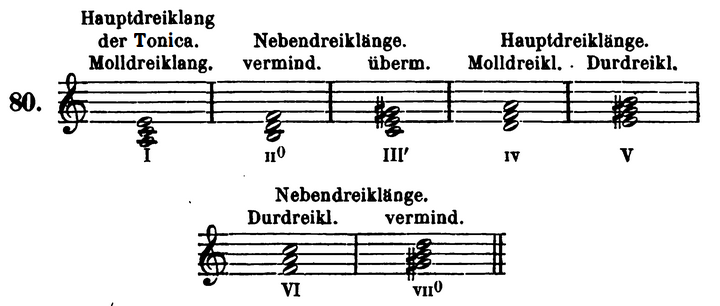
\includegraphics[width=0.6\textwidth]{figures/chapter/2/primary_sources/jadassohn1883lehrbuch038.png}
    \caption{Augmented triads in \textcite{jadassohn1883lehrbuch}, indicated as $\rn{III'}$.}
    \label{fig:jadassohn1883lehrbuch038}
\end{figure}

This syntax of the single-quote augmented triad appeared in at least the treatises by \textcite{broekhoven1889system}, \textcite{buwa1893schule}, and \textcite{shepard1896harmony}.

\begin{figure}
    \centering
    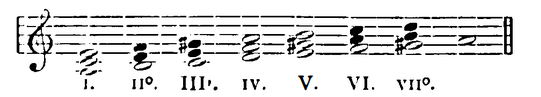
\includegraphics[width=0.6\textwidth]{figures/chapter/2/primary_sources/broekhoven1889system028.png}
    \caption{Augmented triads in \textcite{broekhoven1889system}, using a similar notation to the one found in \textcite{jadassohn1883lehrbuch}.}
    \label{fig:broekhoven1889system028}
\end{figure}

An important component of the modern Roman numeral analysis syntax is the one used for tonicizations.
Tonicizations are slight deviations of key, which usually return to the original key, without ``invoking'' a modulation.
Nowadays, tonicizations are generally written with a slash symbol, where the numerator indicates the scale degree and the denominator indicates the tonicized key.
A common example is $\rn{V/V}$ or (dominant of the dominant).
It is unclear where this notation originally emerged, however, a similar notation was introduced by \textcite{shepard1889how}.
Shepard's notation, which he calls ``[A]ttendant chords'', is presented as ``$\rn{[A] of V}$'' in the notation, shown in Figure~\ref{fig:shepard1889how005}.
This is analogous to $\rn{V/V}$.
An advantage of the modern notation is that other degrees other than $\rn{V}$ (in the numerator) can be annotated using the same syntax.
Piston in fact used Shepard's notation in this way, using a syntax of the form ``$\rn{V of V}$''.
In the explanations of his modulation method, Shepard also introduces a modulation ``formula'' that resembles the fraction-like notation we use today (see Figure~\ref{fig:shepard1889how010}).
Lastly, Shepard included figured bass annotations next to the Roman numeral to indicate certain chord inversions, notably, the cadential six-four chord, as shown in Figure~\ref{fig:shepard1896harmony184}.
This notation was consistent even when there was no music notation involved, where Shepard would write the Arabic numerals next to the Roman numeral in plain-text form, as shown in Figure~\ref{fig:shepard1896harmony117}.

\begin{figure}[h!]
    \centering
    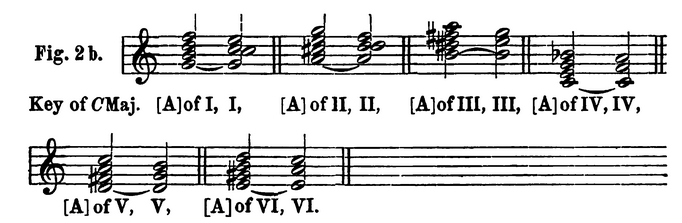
\includegraphics[width=0.6\textwidth]{figures/chapter/2/primary_sources/shepard1889how005.png}
    \caption{Attendant chords in \textcite{shepard1889how}.}
    \label{fig:shepard1889how005}
\end{figure}

\begin{figure}[h!]
    \centering
    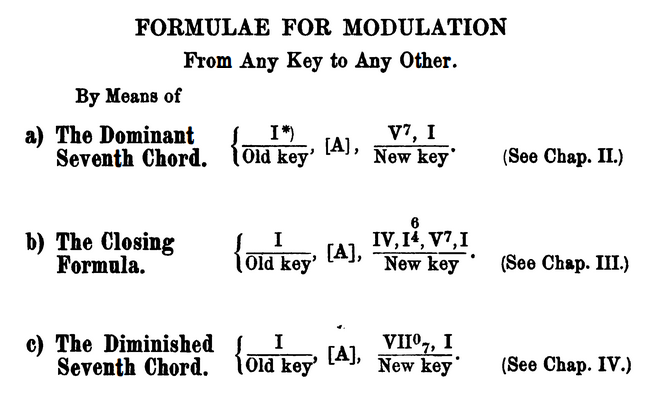
\includegraphics[width=0.6\textwidth]{figures/chapter/2/primary_sources/shepard1889how010.png}
    \caption{Modulation formula in \textcite{shepard1889how}.}
    \label{fig:shepard1889how010}
\end{figure}

\begin{figure}[h!]
    \centering
    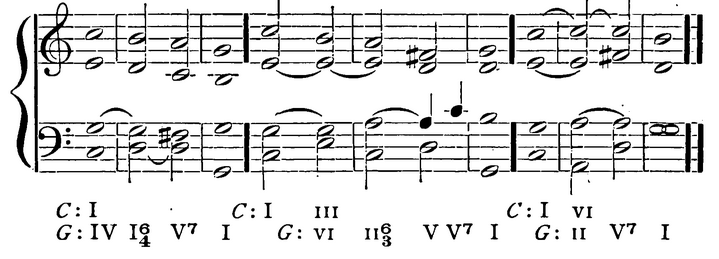
\includegraphics[width=0.6\textwidth]{figures/chapter/2/primary_sources/shepard1896harmony184.png}
    \caption{Shepard's Arabic-numeral inversions \textcite{shepard1896harmony}.}
    \label{fig:shepard1896harmony184}
\end{figure}

\begin{figure}[h!]
    \centering
    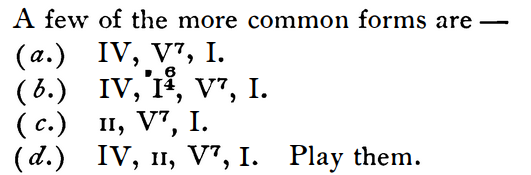
\includegraphics[width=0.6\textwidth]{figures/chapter/2/primary_sources/shepard1896harmony117.png}
    \caption{Shepard's Arabic-numeral inversions \textcite{shepard1896harmony}.}
    \label{fig:shepard1896harmony117}
\end{figure}

Regarding numeric inversions, \textcite{chadwick1897harmony} made this notation explicit. 
Figure~\ref{fig:chadwick1897harmony012} shows his explanation.
This notation goes beyond triads, including for example 
$\rn{V}\rnfourthree$, shown in Figure~\ref{fig:chadwick1897harmony028}.

\begin{figure}[h!]
    \centering
    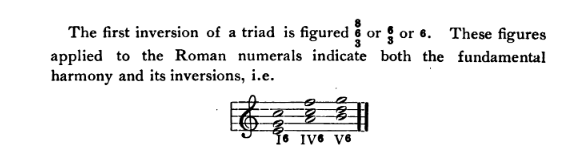
\includegraphics[width=0.6\textwidth]{figures/chapter/2/primary_sources/chadwick1897harmony012.png}
    \caption{Chadwick's Arabic-numeral inversions \textcite{chadwick1897harmony}.}
    \label{fig:chadwick1897harmony012}
\end{figure}

\begin{figure}[h!]
    \centering
    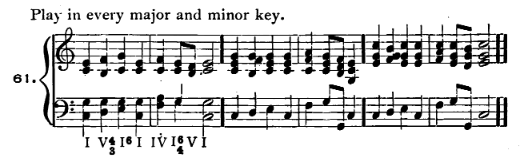
\includegraphics[width=0.6\textwidth]{figures/chapter/2/primary_sources/chadwick1897harmony028.png}
    \caption{A dominant seventh chord in second inversion in \textcite{chadwick1897harmony}.}
    \label{fig:chadwick1897harmony028}
\end{figure}

\begin{figure}[h!]
    \centering
    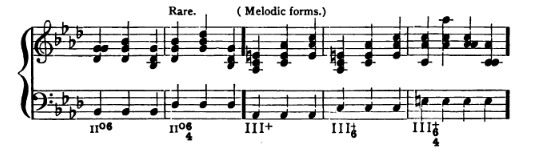
\includegraphics[width=0.6\textwidth]{figures/chapter/2/primary_sources/chadwick1897harmony053.png}
    \caption{The notation for augmented triads in \textcite{chadwick1897harmony}, which is similar to the one by \textcite{riemann1890katechismus}.}
    \label{fig:chadwick1897harmony053}
\end{figure}

\begin{figure}[h!]
    \centering
    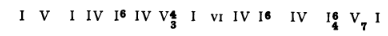
\includegraphics[width=0.6\textwidth]{figures/chapter/2/primary_sources/chadwick1897harmony064.png}
    \caption{\textcite{chadwick1897harmony} describing numeric inversions even in examples without music notation in them.}
    \label{fig:chadwick1897harmony064}
\end{figure}

\begin{figure}[h!]
    \centering
    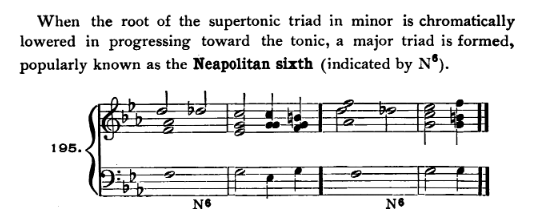
\includegraphics[width=0.6\textwidth]{figures/chapter/2/primary_sources/chadwick1897harmony148.png}
    \caption{Neapolitan in \textcite{chadwick1897harmony}.}
    \label{fig:chadwick1897harmony148}
\end{figure}

Chadwick adopted the Riemann notation for augmented triads, using $\rn{III+}$, as shown in Figure~\ref{fig:chadwick1897harmony053}.
As with Shepard, the numeric inversions are visible even in annotations without any music notation (see Figure~\ref{fig:chadwick1897harmony064}).
Similarly to Emery, Chadwick expressed Neapolitan chords using a special figure $\rn{N}$.
Chadwick was explicit in expressing a Neapolitan as being in first inversion, $\rn{N}\rnsix$, as shown in Figure~\ref{fig:chadwick1897harmony148}.

\textcite{halm1900harmonielehre} can be considered another pioneer of the $\rn{V/V}$ notation.
He used a similar notation $\rn{V--V}$ to refer to secondary dominant chords.
The meaning of this notation is not very clear, because previously he uses it in the form of $\rn{I--V}$ and $\rn{I--IV}$ to denote chords that act as a tonic in one key and as a dominant in another key, but this notation does not work for his $\rn{V--V}$, which should be written as $\sharp{}\rn{II--V}$ or similarly.
Nevertheless, the spirit of the notation is similar to the modern way of thinking about applied chords.
An example of Halm's notation is shown in Figure~\ref{fig:halm1900harmonielehreXVII}

\begin{figure}[h!]
    \centering
    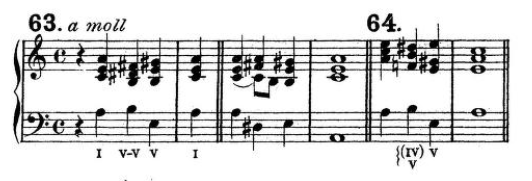
\includegraphics[width=0.6\textwidth]{figures/chapter/2/primary_sources/halm1900harmonielehreXVII.png}
    \caption{Notation for secondary dominants in \textcite{halm1900harmonielehre}.}
    \label{fig:halm1900harmonielehreXVII}
\end{figure}


Another notation for chord inversions adopted by several theorists consists of the use of letters.
In \textcite{cutter1902harmonic}, both notations are explained (see Figure~\ref{fig:cutter1902harmonic004}).

\begin{figure}[h!]
    \centering
    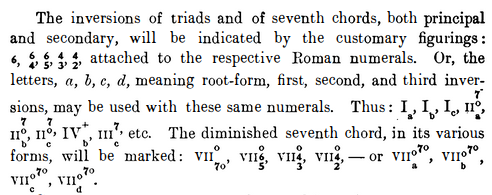
\includegraphics[width=0.6\textwidth]{figures/chapter/2/primary_sources/cutter1902harmonic004.png}
    \caption{Inversions by Arabic numerals and by letters explained in \textcite{halm1900harmonielehre}.}
    \label{fig:cutter1902harmonic004}
\end{figure}

The numeric inversion syntax was already used by previous theorists, however, the letters ${a, b, c , d}$ do not seem to appear before this treatise.
It is also unusual that Cutter mentions both syntaxes in the same work, possibly because this is a treatise on harmonic analysis, rather than a harmony textbook (i.e., harmonization).
Throughout the examples, however, only the numeric inversions are used.

Schenker adopted several notational conventions in \emph{Neue Musikalische Theorien und Phantasien: Harmonielehre} \parencite{schenker1906neue}.
Throughout this book, pivot chords that have multiple meanings in different keys are usually expressed in Roman numerals.
Schenker sometimes uses the notation $\rn{VI=IV}$, and other times $\rn{VI/IV}$.
Some of his specific examples can be seen in Figures \ref{fig:schenker1906neue190}, \ref{fig:schenker1906neue079} and \ref{fig:schenker1906neue190}.

\begin{figure}[h!]
    \centering
    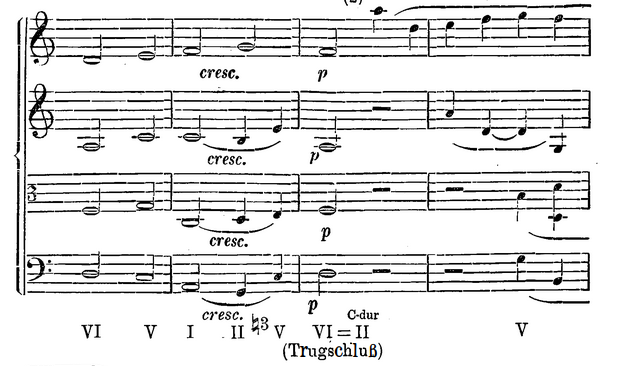
\includegraphics[width=0.6\textwidth]{figures/chapter/2/primary_sources/schenker1906neue078.png}
    \caption{Schenker notation for applied chords.}
    \label{fig:schenker1906neue078}
\end{figure}

\begin{figure}[h!]
    \centering
    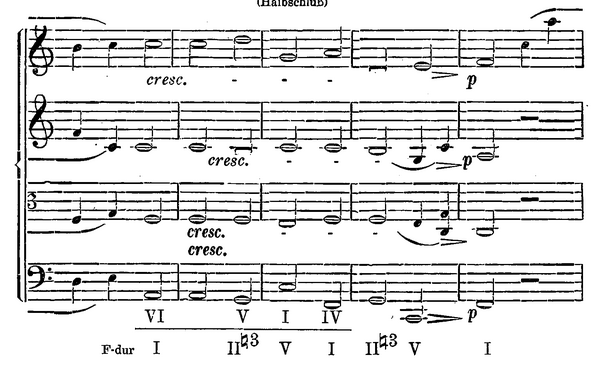
\includegraphics[width=0.6\textwidth]{figures/chapter/2/primary_sources/schenker1906neue079.png}
    \caption{Schenker notation for applied chords.}
    \label{fig:schenker1906neue079}
\end{figure}

\begin{figure}[h!]
    \centering
    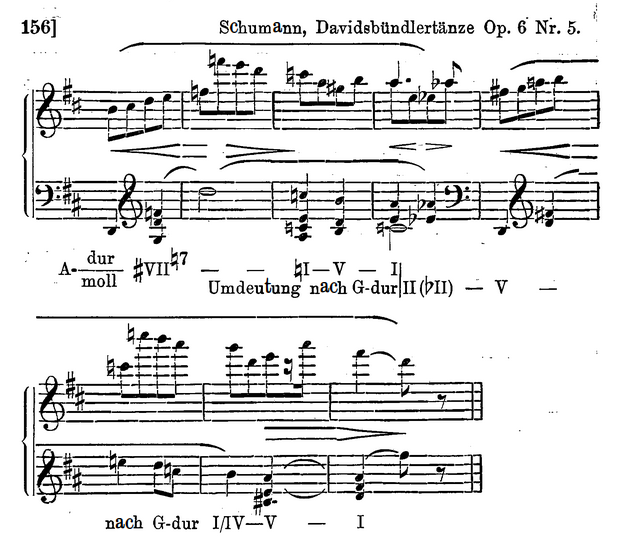
\includegraphics[width=0.6\textwidth]{figures/chapter/2/primary_sources/schenker1906neue190.png}
    \caption{Schenker notation for applied chords.}
    \label{fig:schenker1906neue190}
\end{figure}

The numeric inversion notation could have started, additionally to augmented sixth chords, with cadential six-four chords.
A clear example of this can be seen in \textcite{loewengard1908lehrbuch}, where the cadential six-four figure ($\rn{I}\rnsixfour$) has the numeric inversion notation, but the $\rn{ii}\rnsix$ chord in the same line does not (see Figure~\ref{fig:loewengard1908lehrbuch045}).

\begin{figure}[h!]
    \centering
    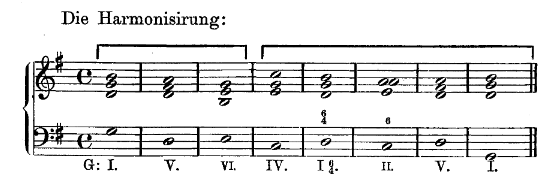
\includegraphics[width=0.6\textwidth]{figures/chapter/2/primary_sources/loewengard1908lehrbuch045.png}
    \caption{Missing first inversion in \textcite{loewengard1908lehrbuch}.}
    \label{fig:loewengard1908lehrbuch045}
\end{figure}

The notation for chord inversions based on letters is less common than the stacks of Arabic numerals.
One place where the letter notation was preferred was \textcite{york1909practical}, where it appears prominently.
Figure~\ref{fig:york1909practical019} shows the introduction of the chord inversion notation used by York.

\begin{figure}[h!]
    \centering
    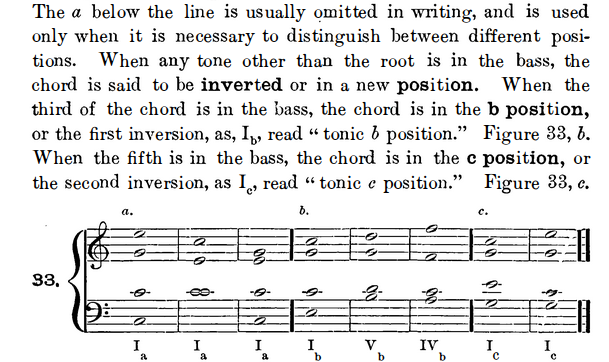
\includegraphics[width=0.6\textwidth]{figures/chapter/2/primary_sources/york1909practical019.png}
    \caption{\textcite{york1909practical}, where the inversion by letter notation is preferred.}
    \label{fig:york1909practical019}
\end{figure}

An interesting notation for secondary dominants appears in \textcite{white1911harmonic}, where it seems to be introduced particularly for diminished seventh chords.
In this notation, secondary dominants are presented within parenthesis, indicating the key they tonicize.
It is clear that these changes of key are different from the other indications of change, like the multirow analysis with a second row of Roman numerals, which permanently change the key in the next chord.
This is consistent with a notation of \emph{tonicizations} and \emph{modulations}, as seen in recent works of computational music theory. 
An example of this notation is shown in Figure~\ref{fig:white1911harmonic110}.

\begin{figure}[h!]
    \centering
    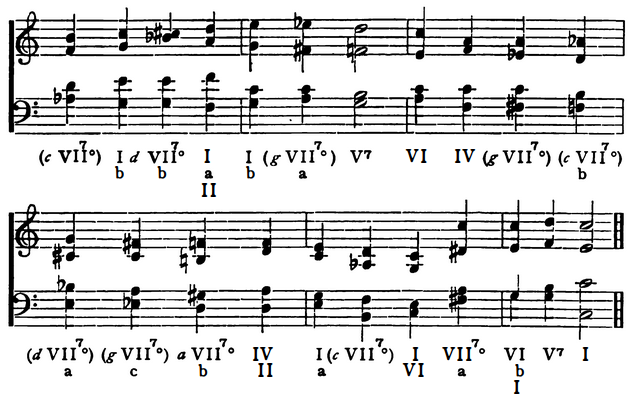
\includegraphics[width=0.6\textwidth]{figures/chapter/2/primary_sources/white1911harmonic110.png}
    \caption{Notation for key fluctuations, in parentheses, appearing in \textcite{white1911harmonic}.}
    \label{fig:white1911harmonic110}
\end{figure}

The notation of $\rn{V of V}$ is observed in \textcite{mokrejs1913lessons}, which is shown in Figure~\ref{fig:mokrejs1913lessons079}.

\begin{figure}[h!]
    \centering
    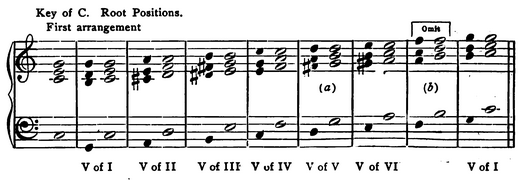
\includegraphics[width=0.6\textwidth]{figures/chapter/2/primary_sources/mokrejs1913lessons079.png}
    \caption{Applied chord syntax in \textcite{mokrejs1913lessons}.}
    \label{fig:mokrejs1913lessons079}
\end{figure}

\textcite{gilson1919traite} presented a numerator/denominator notation of Roman numerals, which is shown in Figure~\ref{fig:gilson1919traite049}.

\begin{figure}[h!]
    \centering
    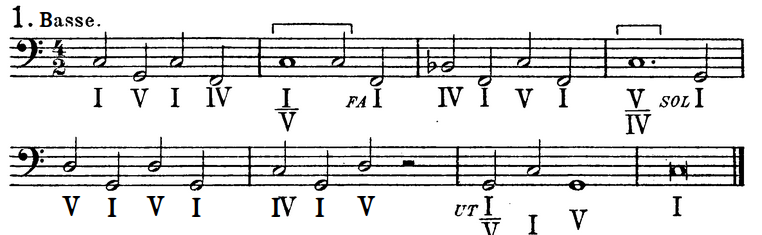
\includegraphics[width=0.6\textwidth]{figures/chapter/2/primary_sources/gilson1919traite049.png}
    \caption{Numerator/denominator notation of Roman numerals in \textcite{gilson1919traite}.}
    \label{fig:gilson1919traite049}
\end{figure}

\begin{figure}[h!]
    \centering
    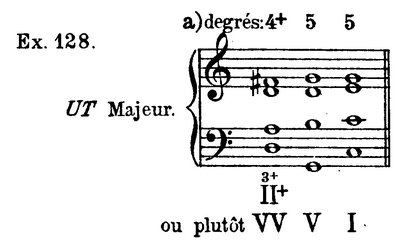
\includegraphics[width=0.6\textwidth]{figures/chapter/2/primary_sources/gilson1919traite090.png}
    \caption{Secondary dominants with $\rn{VV}$ notation in \textcite{gilson1919traite}.}
    \label{fig:gilson1919traite090}
\end{figure}

The Roman numeral notation by Gilson is a mixture of Riemannian functions and scale-degree Roman numerals, an unconventional style in current workflows.
Gilson also introduced the notation $\rn{VV}$ for \emph{dominant of the dominant} chords (see Figure~\ref{fig:gilson1919traite090}).

The Roman numeral syntax seems to be generally less popular among French authors.
For example, Koechlin sporadically uses Roman numerals to indicate scale degrees of only the bass note \textcite{koechlin1928traite}, shown in Figure~\ref{fig:koechlin1928traite026}.

\begin{figure}[h!]
    \centering
    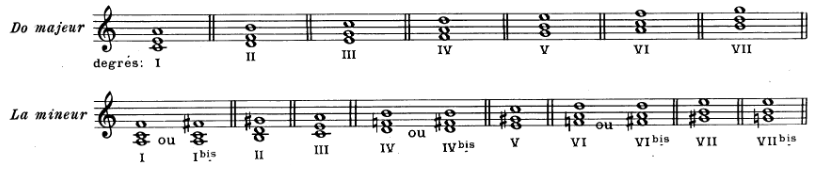
\includegraphics[width=0.6\textwidth]{figures/chapter/2/primary_sources/koechlin1928traite026.png}
    \caption{The scale-degrees of \textcite{koechlin1928traite}, which refer to the only to the bass note and not the root of the chord.}
    \label{fig:koechlin1928traite026}
\end{figure}

This practice is uncommon, as most authors on these days already think in terms of chord roots, not in terms of melodic scale degrees.
In contrast, figured bass notation seemed prominent among French authors.
In some English and German books, they often refer to figured bass as the \emph{French} system.\footnote{For example, \textcite{norris1894practical}}

The modern notation for tonicizations appears in \textcite{tischler1964practical}.

The Shepard notation also shows up in \textcite{goldman1965harmony}.
Goldman also employed the symbols $\rn{Fr}$, $\rn{It}$ and $\rn{German}$ to refer to the augmented sixth chords.